\documentclass{article}

\usepackage{fullpage}
\usepackage{nopageno}
\usepackage{amsmath}
\usepackage{amsfonts}
\usepackage{graphicx}
\usepackage{algorithmic}
\usepackage{xcolor}
\usepackage{framed}

\definecolor{dark_red}{rgb}{0.5,0.0,0.0}

\newcommand{\abs}[1]{\left|#1\right|}
\newcommand{\atan}{\text{atan}}
\newcommand{\rowxyvec}[2]{\left\langle #1, #2 \right\rangle}
\newcommand{\rowvec}[3]{\left\langle #1, #2, #3 \right\rangle}
\newcommand{\colxyvec}[2]{\begin{bmatrix} #1 \\ #2 \end{bmatrix}}
\newcommand{\colvec}[3]{\begin{bmatrix} #1 \\ #2 \\ #3 \end{bmatrix}}
\newcommand{\at}[1]{\left. #1 \right|}
\newcommand{\diff}[2]{\frac{d #1}{d #2}}
\newcommand{\partdiff}[2]{\frac{\partial #1}{\partial #2}}
\newcommand{\mvec}[1]{\overrightarrow{\mathbf{#1}}}
\newcommand{\pvec}[1]{\overrightarrow{#1}}
\newcommand{\dr}[1]{\textcolor{dark_red}{#1}}


\title{Theorems related to Vector Calculus}
\date{}

\begin{document}

\maketitle


%%%%%%%%%%%%%%%%%%%%%%%%%% Question 1
\section*{Question 1:}

\subsection*{part 1a:}

Evaluate the scalar line integral: 

\[\int_C (6x^2 + 4y)ds \quad\text{where}\quad \mathbf{r}_C(t) = \colxyvec{3t + 2}{-t + 3} \;\text{and}\; t \in [-1,1]\]


\subsection*{part 1b:}

Evaluate the scalar line integral: 

\[\int_C (x^2 + 2y)ds \quad\text{where}\quad \mathbf{r}_C(t) = \colxyvec{1 - 2t}{2 - t} \;\text{and}\; t \in [0,3]\]


\subsection*{part 1c:}

Evaluate the scalar line integral: 

\[\int_C 2x \cdot \sin(y) \cdot ds \quad\text{where}\quad \mathbf{r}_C(t) = \colxyvec{\cos(t)}{t} \;\text{and}\; t \in [0,\pi/2]\]




%%%%%%%%%%%%%%%%%%%%%%%%%% Question 2
\section*{Question 2:}

\subsection*{part 2a:}

Evaluate the vector line integral: 

\[\int_C \colxyvec{-6x}{4y} \cdot d\mathbf{r} \quad\text{where}\quad \mathbf{r}_C(t) = \colxyvec{t^2}{1/t} \;\text{and}\; t \in [1,2]\]


\subsection*{part 2b:}

Evaluate the vector line integral: 

\[\int_C \colxyvec{y}{x} \cdot d\mathbf{r} \quad\text{where}\quad \mathbf{r}_C(t) = \colxyvec{t^3}{t^4} \;\text{and}\; t \in [0,2]\]


\subsection*{part 2c:}

Evaluate the vector line integral: 

\[\int_C \colvec{2x}{y^2}{-z} \cdot d\mathbf{r} \quad\text{where}\quad \mathbf{r}_C(t) = \colvec{-t^2}{t+4}{3t+2} \;\text{and}\; t \in [-1,1]\]




%%%%%%%%%%%%%%%%%%%%%%%%%% Question 3
\section*{Question 3:}

\subsection*{part 3a:}

Is the vector field \(\mathbf{F}(x,y,z) = \colvec{y^2\sin(z)}{2xy\sin(z)}{xy^2\cos(z)}\) conservative? If yes, use the {\bf gradient theorem} to evaluate the vector line integral:

\[\int_C \colvec{y^2\sin(z)}{2xy\sin(z)}{xy^2\cos(z)} \cdot d\mathbf{r} \quad\text{where}\quad \mathbf{r}_\text{initial} = \colvec{0}{0}{0} \;\text{and}\; \mathbf{r}_\text{final} = \colvec{1}{1}{\pi/2}\] 


\subsection*{part 3b:}

Is the vector field \(\mathbf{F}(x,y,z) = \colvec{xy}{xy}{z}\) conservative? If yes, use the {\bf gradient theorem} to evaluate the vector line integral:

\[\int_C \colvec{xy}{xy}{z} \cdot d\mathbf{r} \quad\text{where}\quad \mathbf{r}_\text{initial} = \colvec{0}{0}{0} \;\text{and}\; \mathbf{r}_\text{final} = \colvec{1}{1}{1}\] 




%%%%%%%%%%%%%%%%%%%%%%%%%% Question 4
\section*{Question 4:}

\subsection*{part 4a:}

\begin{tabular}{cc}
\parbox{0.6\textwidth}{ 
The region \(\sigma\) on the right is 
\[\sigma = \{(x,y) | 0 \leq x \leq 6 \;\text{and}\; 0 \leq y \leq 3 - (1/2)x\}\]
Use Green's theorem to compute the loop integral
\[\int_{\partial\sigma} \colxyvec{3x-5y}{x-2y} \cdot d\mathbf{r}\]
where \(\partial\sigma\) is the counterclockwise oriented boundary of \(\sigma\).
} & \parbox{0.4\textwidth}{
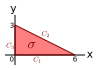
\includegraphics[width = 0.4\textwidth]{Test_bench_part_4x_images/Test_bench_part_4x_image_1}
}
\end{tabular}
Next, compute each of \(\int_{C_1} \colxyvec{3x-5y}{x-2y} \cdot d\mathbf{r}\); \(\int_{C_2} \colxyvec{3x-5y}{x-2y} \cdot d\mathbf{r}\); and \(\int_{C_3} \colxyvec{3x-5y}{x-2y} \cdot d\mathbf{r}\) and show that 
\[\int_{\partial\sigma} \colxyvec{3x-5y}{x-2y} \cdot d\mathbf{r} = \int_{C_1} \colxyvec{3x-5y}{x-2y} \cdot d\mathbf{r} + \int_{C_2} \colxyvec{3x-5y}{x-2y} \cdot d\mathbf{r} + \int_{C_3} \colxyvec{3x-5y}{x-2y} \cdot d\mathbf{r}\]  



\subsection*{part 4b:}

\begin{tabular}{cc}
\parbox{0.6\textwidth}{ 
The region \(\sigma\) on the right is 
\[\sigma = \{(x,y) | 0 \leq x \leq 1 \;\text{and}\; x^3 \leq y \leq x\}\]
Use Green's theorem to compute the loop integral
\[\int_{\partial\sigma} \colxyvec{2xy}{x+y} \cdot d\mathbf{r}\]
where \(\partial\sigma\) is the counterclockwise oriented boundary of \(\sigma\).
} & \parbox{0.4\textwidth}{
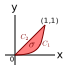
\includegraphics[width = 0.4\textwidth]{Test_bench_part_4x_images/Test_bench_part_4x_image_2}
}
\end{tabular}
Next, compute each of \(\int_{C_1} \colxyvec{2xy}{x+y} \cdot d\mathbf{r}\); and \(\int_{C_2} \colxyvec{2xy}{x+y} \cdot d\mathbf{r}\) and show that 
\[\int_{\partial\sigma} \colxyvec{2xy}{x+y} \cdot d\mathbf{r} = \int_{C_1} \colxyvec{2xy}{x+y} \cdot d\mathbf{r} + \int_{C_2} \colxyvec{2xy}{x+y} \cdot d\mathbf{r}\]  



\subsection*{part 4c:}

\begin{tabular}{cc}
\parbox{0.6\textwidth}{ 
The region \(\sigma\) on the right is 
\[\sigma = \{(x,y) | -4 \leq x \leq 0 \;\text{and}\; 0 \leq y \leq 2 + (1/2)x\}\]
Use Green's theorem to compute the loop integral
\[\int_{\partial\sigma} \colxyvec{x+2y}{5x+y} \cdot d\mathbf{r}\]
where \(\partial\sigma\) is the counterclockwise oriented boundary of \(\sigma\).
} & \parbox{0.4\textwidth}{
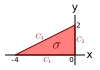
\includegraphics[width = 0.4\textwidth]{Test_bench_part_4x_images/Test_bench_part_4x_image_3}
}
\end{tabular}
Next, compute each of \(\int_{C_1} \colxyvec{x+2y}{5x+y} \cdot d\mathbf{r}\); \(\int_{C_2} \colxyvec{x+2y}{5x+y} \cdot d\mathbf{r}\); and \(\int_{C_3} \colxyvec{x+2y}{5x+y} \cdot d\mathbf{r}\) and show that 
\[\int_{\partial\sigma} \colxyvec{x+2y}{5x+y} \cdot d\mathbf{r} = \int_{C_1} \colxyvec{x+2y}{5x+y} \cdot d\mathbf{r} + \int_{C_2} \colxyvec{x+2y}{5x+y} \cdot d\mathbf{r} + \int_{C_3} \colxyvec{x+2y}{5x+y} \cdot d\mathbf{r}\]  




%%%%%%%%%%%%%%%%%%%%%%%%%% Question 5 
\section*{Question 5:}

\begin{tabular}{cc}
\parbox{0.6\textwidth}{ 
The region \(\sigma\) on the right is 
\[\sigma = \{(x,y) | 0 \leq x \leq 1 \;\text{and}\; 0 \leq y \leq 1 - x^2\}\]
Use Gauss's divergence theorem to compute the flux integral
\[\int_{\partial\sigma} \colxyvec{x^2}{y} \cdot \colxyvec{dy}{-dx}\]
where \(\partial\sigma\) is the counterclockwise oriented boundary of \(\sigma\).
} & \parbox{0.4\textwidth}{
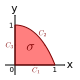
\includegraphics[width = 0.4\textwidth]{Test_bench_part_4x_images/Test_bench_part_4x_image_4}
}
\end{tabular}
Next, compute each of \(\int_{C_1} \colxyvec{x^2}{y} \cdot \colxyvec{dy}{-dx}\); \(\int_{C_2} \colxyvec{x^2}{y} \cdot \colxyvec{dy}{-dx}\); and \(\int_{C_3} \colxyvec{x^2}{y} \cdot \colxyvec{dy}{-dx}\) and show that 
\[\int_{\partial\sigma} \colxyvec{x^2}{y} \cdot \colxyvec{dy}{-dx} = \int_{C_1} \colxyvec{x^2}{y} \cdot \colxyvec{dy}{-dx} + \int_{C_2} \colxyvec{x^2}{y} \cdot \colxyvec{dy}{-dx}+ \int_{C_3} \colxyvec{x^2}{y} \cdot \colxyvec{dy}{-dx}\]  



\end{document}









